\section{Deterministic finite state automata}

\paragraph*{Deterministic finite automaton}
A finite deterministic automaton $M$ consist of five elements:
\begin{enumerate}
    \item $Q$, the state set (finite and not empty). 
    \item $\Sigma$, the input or terminal alphabet
    \item $\delta:(Q \times \Sigma) \rightarrow Q$, the transition function.
    \item $q_0 \in Q$, the initial state. 
    \item $F\subseteq Q$, the set of final states.
\end{enumerate}

\paragraph*{Moves}
The transition function captures the moves of the automaton as follows:
\[\delta(q_i,a)=q_j\]
This notation signifies that when the automaton, denoted as $M$, is in the current state $q_i$ and encounters the input symbol $a$, it transitions the current state to $q_j$. 
If $\delta(q_i, a)$ is undefined, the automaton enters an error state, leading to the rejection of the input string.
The general transition function operates over the domain $Q \times \Sigma^{*}$ and is defined as:
\[\delta(q,ya)=\delta(\delta(q,y),a) \qquad \textnormal{where } a \in \Sigma \textnormal{ and }y \in \Sigma^{*}\]
\begin{definition}[\textit{Recognized string}]
    A string is recognized if, and only if, as the automaton traverses a path labeled by $x$, it commences from the initial state and concludes at one of the final states:
    \[\delta(q_0,x) \in F\]
\end{definition}
It is noteworthy that the empty string is accepted only when the initial state is also a final state.
\begin{definition}[\textit{Finite-state recognizable automata}]
    The languages accepted by such automata are termed finite-state recognizable:
    \[L(M)=\{x \in \Sigma^{*}|x \textnormal{ is recognized by } M\}\]
\end{definition}
\begin{definition}[\textit{Equivalent automata}]
    Two automata are considered equivalent if they accept the same language.
\end{definition}
The time complexity of finite state automata is optimal: the input string $x$ is either accepted or rejected in real-time. 
Since scanning the string from left to right requires precisely as many steps, the recognition time complexity cannot be further reduced.

\subsection{Error state and total automata}
In case the move is not specified in state $q$ when processing character $a$, the automaton enters the error state $q_{\text{err}}$:
\[\forall q \in Q \forall a \in \Sigma \textnormal{ if } \delta(q,a) \textnormal{ is undefined then set } \delta(q,a)=q_{\text{err}}\]
Augmenting the deterministic automaton by introducing the error state is always feasible without altering the accepted language.

\subsection{Clean automata}
An automaton might contain components that do not contribute to any accepting computation and are therefore best removed.
\begin{definition}[\textit{Reachable state}]
    A state $q$ is considered reachable from state $p$ if there exists a computation that transitions from $p$ to $q$.
\end{definition}
\begin{definition}[\textit{Accessible state}]
    A state is accessible if it can be reached from the initial state. 
\end{definition}
\begin{definition}[\textit{Post-accessible state}]
    A state is post-accessible if a final state can be reached from it. 
\end{definition}
\begin{definition}[\textit{Useful state}]
    A state is called useful if it is both accessible and post-accessible.
\end{definition}
\begin{definition}[\textit{Clean automaton}]
    An automaton is deemed  clean if every state within it is useful.
\end{definition}
\begin{property}
    Every finite state automaton has an equivalent clean form.
\end{property}    
To reduce an automaton, the process involves first identifying all the useless states and subsequently removing them from the automaton along with all their incoming and outgoing arcs.




\subsection{Minimal automata}
\begin{property}
    Every finite state language possesses a unique deterministic finite state recognizer with the minimum possible number of states, known as the minimal automaton.
\end{property}   
\begin{definition}[\textit{Undistinguishable states}]
    The states $p$ and $q$ are undistinguishable if, and only if, for every string $x \in \Sigma^{*}$, either both states $\delta(p,x)$ and $\delta(q,x)$ are final, or neither is final.
\end{definition}
The merging of two indistinguishable states allows for a reduction in the number of states in the automaton without altering the recognized language.
Undistinguishability is a relation that is symmetric, reflexive, and transitive.
\begin{definition}[\textit{Distinguishable states}]
    The states $p$ and $q$ are distinguishable if, and only if $p$ is final and $q$ is not, and $\delta(p,a)$ is distinguishable from $\delta(q,a)$.
\end{definition}
\begin{example}
    Consider the following deterministic automaton: 
    \begin{figure}[H]
        \centering
        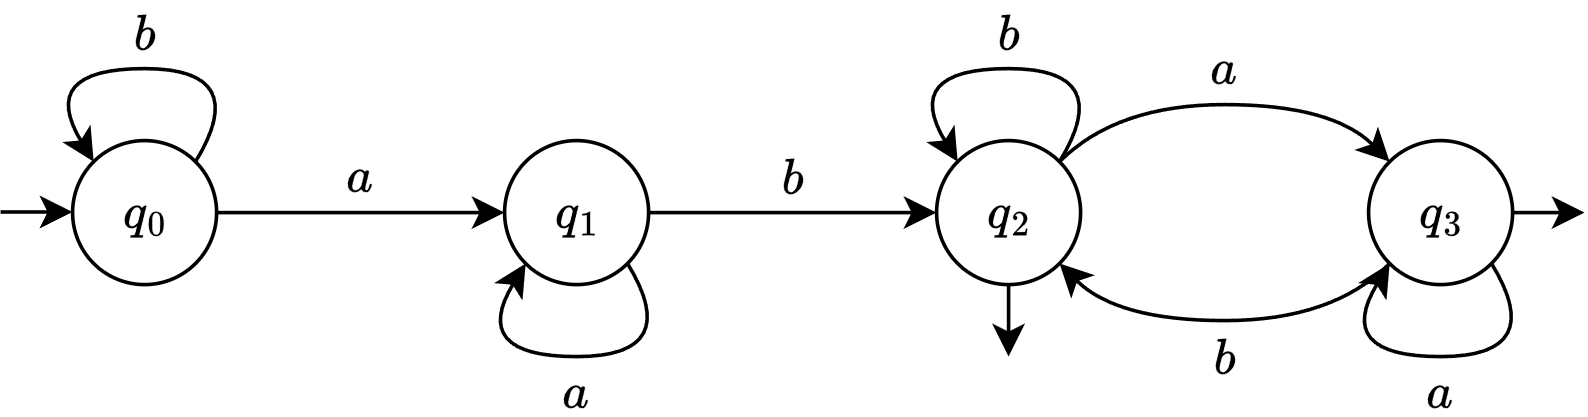
\includegraphics[width=0.75\linewidth]{images/fsamin.png}
    \end{figure}
    The corresponding undistinguishability table is as follows: 
    \begin{table}[H]
        \centering
        \begin{tabular}{cclcccc}
        \cline{2-3}
        \multicolumn{1}{c|}{\multirow{2}{*}{$q_1$}} & \multicolumn{2}{c|}{(1,1)}                     &                        &                       &              &             \\
        \multicolumn{1}{c|}{}                       & \multicolumn{2}{c|}{(0,2)}                     &                        &                       &              &             \\ \cline{2-5}
        \multicolumn{1}{c|}{\multirow{2}{*}{$q_2$}} & \multicolumn{2}{c|}{\multirow{2}{*}{$\times$}} & \multicolumn{2}{c|}{\multirow{2}{*}{$\times$}} &              &             \\
        \multicolumn{1}{c|}{}                       & \multicolumn{2}{c|}{}                          & \multicolumn{2}{c|}{}                          &              &             \\ \cline{2-7} 
        \multicolumn{1}{c|}{\multirow{2}{*}{$q_1$}} & \multicolumn{2}{c|}{\multirow{2}{*}{$\times$}} & \multicolumn{2}{c|}{\multirow{2}{*}{$\times$}} & \multicolumn{2}{c|}{(3,3)} \\
        \multicolumn{1}{c|}{}                       & \multicolumn{2}{c|}{}                          & \multicolumn{2}{c|}{}                          & \multicolumn{2}{c|}{(2,2)} \\ \cline{2-7} 
                                                    & \multicolumn{2}{c}{$q_1$}                      & \multicolumn{2}{c}{$q_2$}                      & \multicolumn{2}{c}{$q_3$} 
        \end{tabular}
    \end{table}
    From the table, it is evident that the only indistinguishable states are $q_2$ and $q_3$.
\end{example}

\paragraph*{Minimization}
The minimal automaton $M^{'}$, equivalent to the given automaton $M$ has states corresponding to the equivalence classes of the undistinguishability relation.
Defining the transition function of  $M^{'}$ involves stating that there exists an arc from class $C_1=[\dots,p_r,\dots]$ to class $C_2=[\dots,q_s,\dots]$ if and only if in $M$, there is an arc from state $p_r$ to $q_s$ with the same label:
\[p_r \overset{b}{\rightarrow}q_s \Leftrightarrow C_1=[\dots,p_r,\dots] \overset{b}{\rightarrow} C_2=[\dots,q_s,\dots]\]
In other words, there is an arc between two states belonging to the two classes.
\begin{example}
    Consider the automaton from the previous example; it can be minimized by merging the two indistinguishable states found in the undistinguishability table.
    The resulting minimized automaton is as follows:
    \begin{figure}[H]
        \centering
        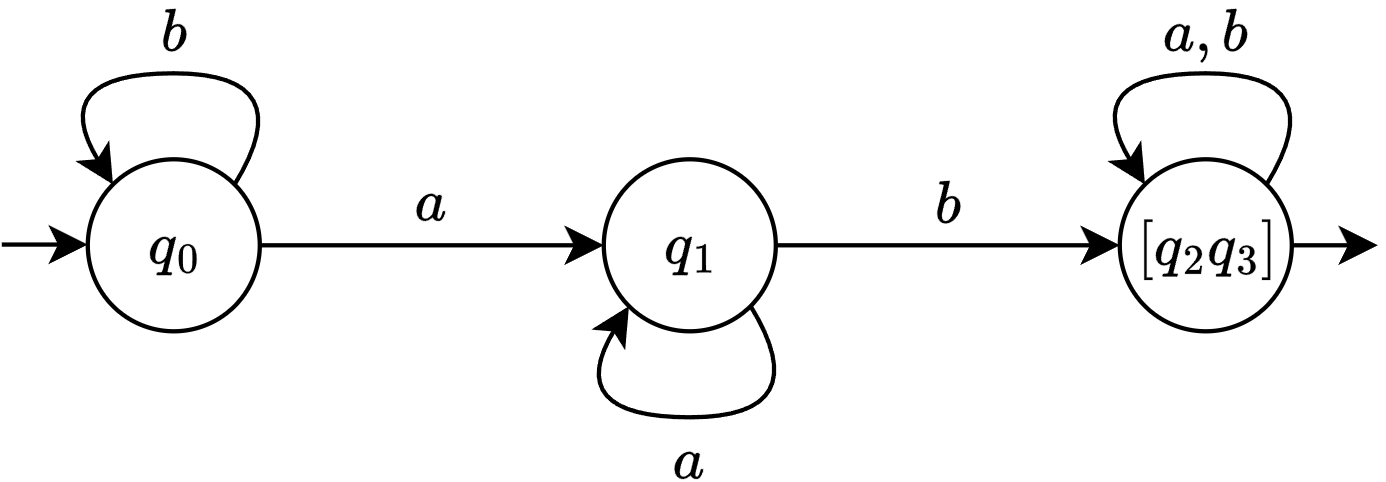
\includegraphics[width=0.6\linewidth]{images/fsamin1.png}
    \end{figure}
\end{example}